\hypertarget{immersion-culturelle-uxe0-mexico-city}{%
\section{Immersion culturelle à Mexico
City}\label{immersion-culturelle-uxe0-mexico-city}}

\emph{Dimanche 30 septembre 2018}

Deux semaines n'étaient pas de trop pour découvrir l'immense capitale du
Mexique et ses alentours. J'ai choisi de séparer le séjour en deux
articles, et celui-ci va être focalisé sur la ville elle-même, récemment
renommée CDMX : Ciudad de México. La suite est
\href{/excursions-mexico.html}{ici}.

\begin{figure}
\centering
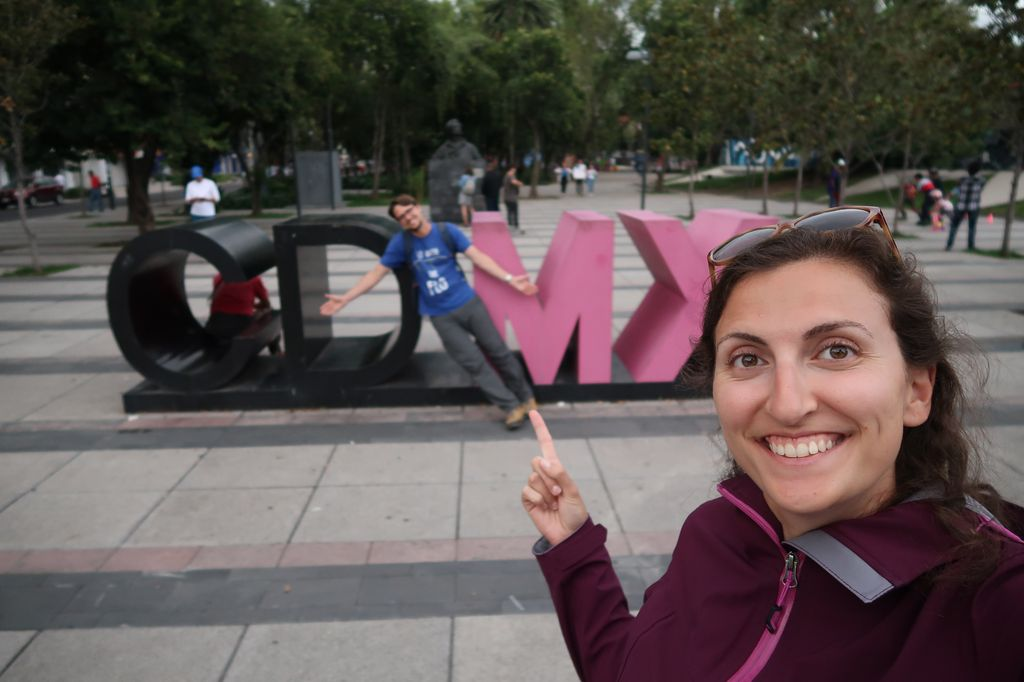
\includegraphics{images/20180930_cdmx.JPG}
\caption{Le logo de la municipalité de Mexico figure un peu partout dans
le paysage urbain.}
\end{figure}

Nous sommes arrivés avec beaucoup d'appréhension et d'\emph{a priori} :
comment va-t-on se déplacer dans cette ville immense ? Quels sont les
quartiers à éviter ? Quid de l'insécurité qui peut faire la mauvaise
réputation de la ville ? Et tous ces doutes se sont progressivement
effacés, pour laisser place à l'émerveillement. Ce qui nous aura surtout
marqué, c'est la puissance culturelle de la ville. Mexico serait la
ville contenant le plus de musées au monde, et ceux-ci sont toujours en
ébullition. Sur le plan musical on a eu la bonne surprise de tomber de
manière quasi-quotidienne sur des concerts gratuits de grande qualité,
un peu partout dans la ville.

Pour prendre nos repères, on a commencé par...un \emph{free walking
tour}, pour changer ! Même \textbf{des} \emph{free walking tours} : on a
visité avec les adorables jeunes guides d'Estacion Mexico le centre
ville, le quartier de Coyoacan, les hauts lieux du muralisme et de la
lucha libre !

Au centre ville, on a découvert le Zocalo et sa cathédrale, mais surtout
le Templo Mayor des aztèques. Ses fondations ont été posées là où les
aztèques ont vu, après 200 ans de migration depuis le Nord du pays, le
symbole divin du lieu de leur nouvelle capitale : un aigle dévorant un
serpent, posé sur le haut d'un cactus (et devinez ce qu'il y a au centre
du drapeau mexicain...). La structure du Templo Mayor, bien que
largement détruit par les espagnols, est faite de 7 pyramides
construites comme des poupées russes, la plus récente englobant la
précédente, \emph{et caetera}. On a aussi découvert que Mexico est une
ville qui coule (de 25 à 40 centimètres par an selon les lieux et les
sources !). Parce que le fameux cactus, il était sur une petite île. Au
milieu d'un lac. Et ça a découragé personne, ni les aztèques, ni les
espagnols qui ont asséché le bassin de la ville pour l'étendre. Et les
conséquences sont bien visibles : les cathédrales et les immeubles
penchent, de manière plus ou moins impressionnante. Ou encore le fait
qu'on a trébuché un nombre incalculable de fois à cause des trottoirs
inclinés de la ville \^{}\^{}.

\begin{figure}
\centering
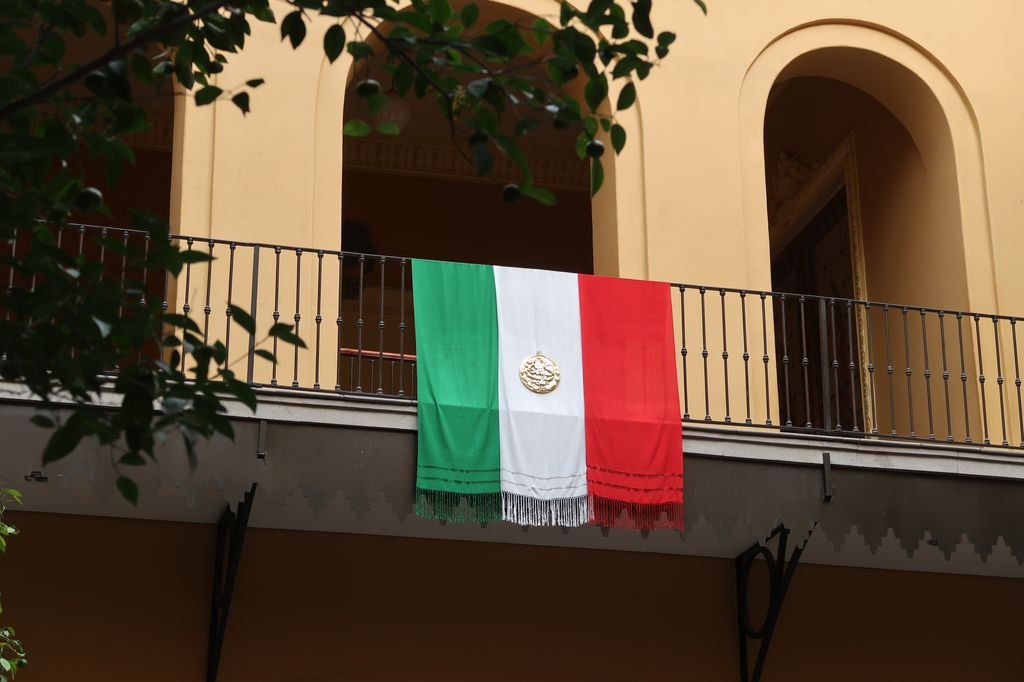
\includegraphics{images/20180930_drapeau.JPG}
\caption{Regardez bien ce qui figure au centre de ce drapeau !}
\end{figure}

L'art du muralisme nous a particulièrement impressionné : ces grandes
fresques peintes dans des lieux publics (universités, ministères, palais
des Beaux-Arts, palais national) étaient destinées à enseigner
l'Histoire du pays à un public qui était, à l'époque de la révolution
mexicaine, majoritairement illettré. Et ça a donné des œuvres
monumentales, dont celles du célèbre Diego Rivera, mari de Frida Kahlo.

Dans le quartier de Coyoacan, où ils ont vécu, on en a justement appris
plus sur ce sulfureux couple que formaient Frida et Diego (une très
longue histoire de je-t-aime-moi-non-plus qui donne le vertige rien que
d'y repenser). On y a aussi flâné dans les rues colorées un churros à la
main (bisous Raph ;) ), on s'est perdus dans le marché (on trouve pas la
sortie ? bon bah on va manger des tacos alors \^{}\^{}), et on a admiré
les riches décorations encore en place de la fête nationale quelques
jours auparavant...

\begin{figure}
\centering
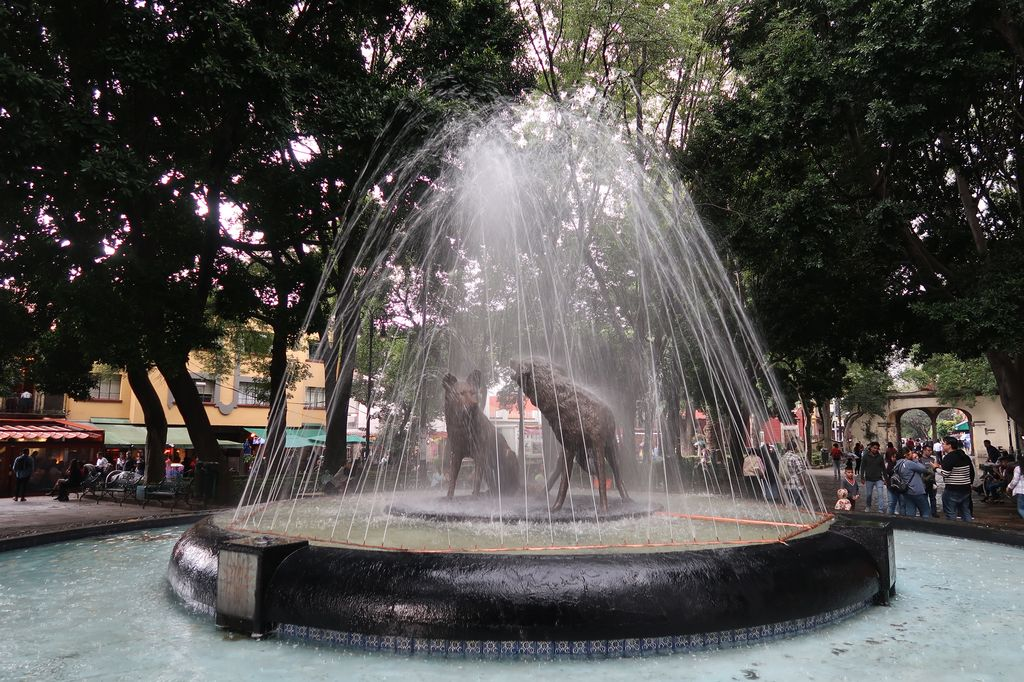
\includegraphics{images/20180930_coyoacan.JPG}
\caption{Devinez-vous pourquoi le quartier se nomme Coyoacan ?}
\end{figure}

Pour le côté culture populaire, on a été très agréablement surpris par
les soirées de \emph{lucha libre}. Les combats sont de vrais spectacles
d'acrobates complètement dégénérés (dont certains ont facilement plus de
60 ans !), avec des entrées sur "scène" très travaillées : costumes
hauts en couleurs, musique à fond, photos et vidéos du combattant sur
grand écran, jeunes danseuses de part et d'autre de l'escalier... et
même si sur le ring on comprend que les règles sont bien définies, dans
l'arène tout est permis : c'est une bière dans une main, des pop-corns
dans l'autre que tout le monde crie des insultes bien bien méchantes à
l'égard des combattants. On a même assisté à un moment rare quand l'un
des combattants, Mistico, s'est fait retirer son masque par son
adversaire : fin du match, victoire instantanée de l'adversaire et honte
ultime pour celui qui sort de l'arène le visage caché dans ses mains.
Après une première expérience avec une guide, on y est même retournés
une deuxième fois seuls tellement c'était captivant !

\begin{figure}
\centering
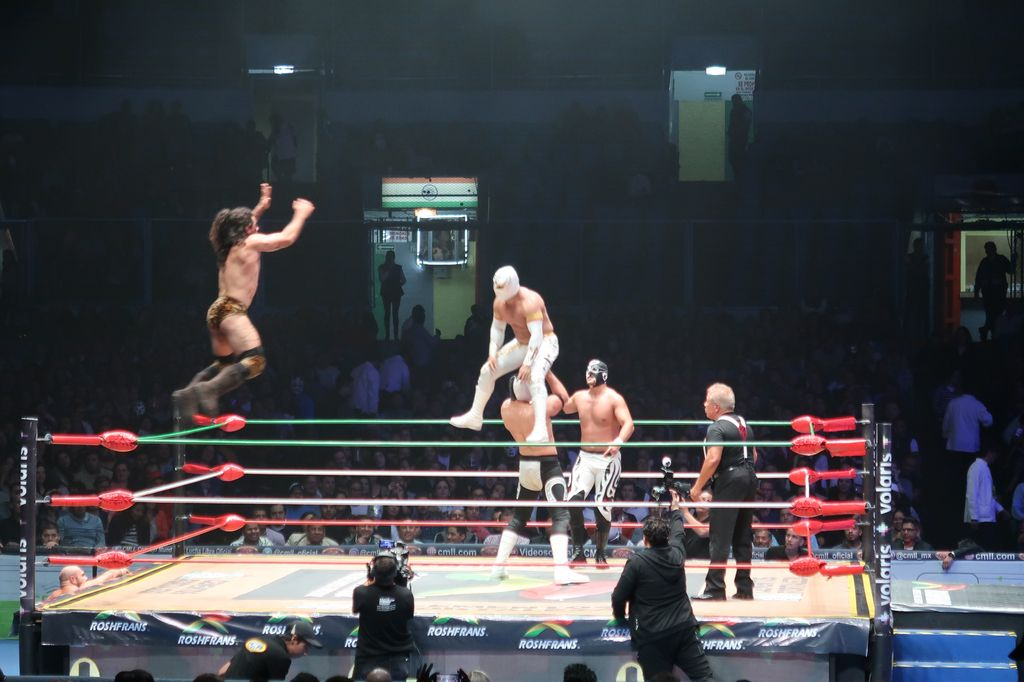
\includegraphics{images/20180930_luchalibre.JPG}
\caption{Spectacle, spectacle et encore du spectacle : la lucha libre.}
\end{figure}

On a aussi passé une soirée dans le quartier des \emph{mariachis}, à la
place Garibaldi. Ces groupes de musiciens interprètent des classiques de
la musique mexicaine à la demande (et sans oublier de payer pour chaque
chanson à la fin). On a eu de la chance de s'installer juste à côté
d'une table de jeunes mexicains bien imbibés qui se sont montrés très
généreux avec les mariachis pour séduire la tablée de touristes d'en
face. Nous, on était aux premières loges pour profiter du spectacle avec
nos cocktails !

Nous avons consacré une journée à l'agréable parc de Chapultepec, centré
sur son "château" aux multiples usages, dont celui de demeure de
l'Empereur de courte durée du Mexique, parachuté là par Napoléon III.
Mais ce qu'on y a préféré, c'est le merveilleux musée d'anthropologie,
où après deux visites il nous restait encore le double de salles à
découvrir !

Dernière curiosité à CDMX, on a passé deux heures sur une
\emph{trajinera} (une sorte de grosse gondole) à naviguer sur les canaux
entre les nombreuses \emph{chinampas} (îles artificielles) où se
succèdent des zones cultivées et des maisons. Ces structures témoignent
de ce qu'était la région avant l'arrivée des espagnols : des villes sur
un grand lac avec des quartiers flottants et des ponts pour relier les
différents endroits, le tout à 2000 mètres d'altitude !

\begin{figure}
\centering
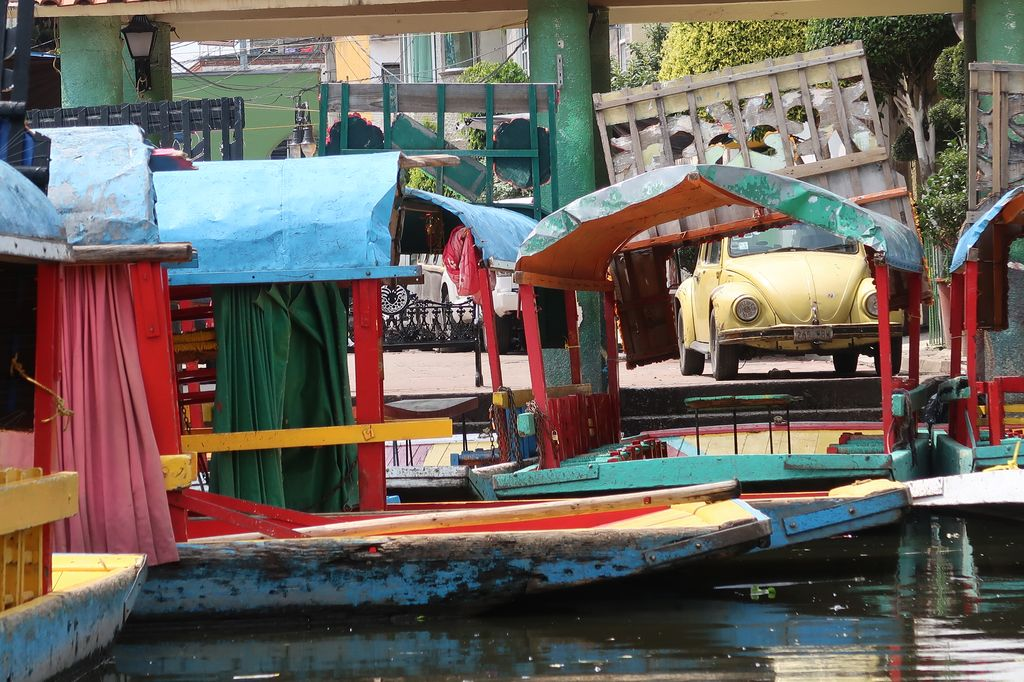
\includegraphics{images/20180930_xochimilco.JPG}
\caption{Ambiance typique à Xochimilco - on aperçoit une Cox' dans le
fond.}
\end{figure}

Après toutes ces belles choses, on en voulait encore plus ! On s'est
donc lancés dans quelques excursions en dehors de la ville : à suivre :)

\emph{Elida}
